\documentclass[a4paper, 10pt, final, garamond]{book}
\usepackage{cours-preambule}
\graphicspath{{./figures/}}

\makeatletter
\renewcommand{\@chapapp}{Contr\^ole de connaissances}
\makeatother

% \toggletrue{student}
% \HideSolutionstrue

\begin{document}
\setcounter{chapter}{3}

\chapter{Électrocinétique~: premier ordre et harmonique}

\ifstudent{
	\begin{tikzpicture}[remember picture, overlay]
		\node[anchor=north west, align=left]
		at ([shift={(1.4cm,0)}]current page.north west)
		{\\[5pt]\Large\bfseries Nom~:\\[10pt]\Large\bfseries Prénom~:};
		\node[anchor=north east, align=right]
		at ([shift={(-1.5cm,-17pt)}]current page.north east)
		{\Large\bfseries Note~:\hspace{1cm}/10};
	\end{tikzpicture}
}

\begin{enumerate}[label=\sqenumi, leftmargin=10pt]
	\nitem{5}
	\noindent
	\begin{minipage}[t]{.69\linewidth}
		On suppose le circuit LC série suivant, en régime libre. On suppose le
		condensateur initialement chargé à la tension $E$, et on ferme l'interupteur
		à $t=0$. Déterminer l'équation différentielle sous forme canonique de $u_C$
		pour $t \geq 0$, donner les conditions initiales et comment les déterminer,
		et résoudre l'équation différentielle pour trouver $u_C(t)$ \textbf{et}
		$i(t)$.
	\end{minipage}
	\hfill
	\begin{minipage}[t]{.29\linewidth}
		~
		\vspace{-30pt}
		\begin{center}
			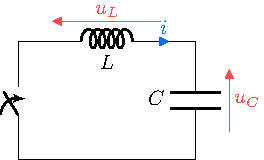
\includegraphics[width=.8\linewidth]{lc_descendant-intens}
			\captionof{figure}{}
		\end{center}
	\end{minipage}
	\begin{isd}[sidebyside align=top]
		\wsw{
			Avec la loi des mailles,
			\begin{DispWithArrows*}[fleqn, mathindent=4em]
				u_L + u_C &= 0
				\Arrow{$u_L = L \dv{i}{t}$\\ et $i = C \dv{u_C}{t}$}
				\\\Lra
				LC \dv[2]{u_C}{t} + u_C          &= 0
				\Arrow{forme canonique}
				\\
				\Lra \dv[2]{u_C}{t} + \frac{1}{LC}u_C &= 0
			\end{DispWithArrows*}
			L'équation homogène est, avec $\w_0 = 1/\sqrt{LC}$~:
			\[
				\boxed{\dv[2]{u_C}{t} + \w_0{}^2u_C = 0}
			\]
			La forme générale de la solution pour cette équation est~:
			\[
				u_C(t) = A\cos(\w_0 t) + B\sin(\w_0 t)
			\]
		}
		\tcblower
		\wsw{
			On trouve $A$ avec la première condition initiale~:
			\[
				u_C(0) = A\cos(0) + B\sin(0) = \boxed{A = E}
			\]
			On trouve $B$ avec la seconde condition initiale~:
			\begin{gather*}
				\dv{u_C}{t} = -A\w_0\sin(\w_0t) + B\w_0\cos(\w_0t)
				\Ra \dv{u_C}{t}\/(0) = B\w_0
				\\
				\text{et} \quad
				i(0) = 0 = C \dv{u_C}{t}\/(0) = CB\w_0
				\quad \Ra \boxed{B = 0}
			\end{gather*}
			D'où
			\[
				\boxed{u_C(t) = E\cos(\w_0t)}
			\]
			On obtient ensuite $i$ avec la relation courant-tension~:
			\[
				\boxed{i(t) = C \dv{u_c}{t} = -CE \w_0 \sin(\w_0t)}
			\]
		}
		\vspace{-15pt}
	\end{isd}
	\nitem{3} Faire un bilan d'énergie pour le circuit LC libre, et montrer que
	l'énergie est conservée à chaque instant. Tracer $\Ec_C$, $\Ec_L$ et
  $\Ec_{\tot}$.
	\smallbreak
	\begin{isd}[righthand ratio=.3]
		\wsw{
			On fait un bilan de puissances avec la loi des mailles multipliée par
			$i$~:
			\begin{DispWithArrows*}
				u_Ci + u_Li &= 0
				\Arrow{$i = C \dv{u_C}{t}$\\et $u_L = L \dv{i}{t}$}
				\\
				\Lra
				u_C\times C \dv{u_C}{t} + L \dv{i}{t}\times i &= 0
				\Arrow{$f \times f' = \left( \frac{1}{2}f^{2} \right)'$}
				\\\Lra
				\dv{}{t} \Big(
				\underbracket[1pt]{\frac{1}{2}Cu_C{}^2}_{=\Ec_C} +
				\underbracket[1pt]{\frac{1}{2}Li^2}_{=\Ec_L}
				\Big) &= 0
				\Arrow{$\Ec_{\tot} = \Ec_C + \Ec_L$}
				\\\Lra
        \Aboxed{\dv{\Ec_{\tot}}{t} = 0}
			\end{DispWithArrows*}
			L'énergie totale est bien conservée.
		}
		\tcblower
		\begin{center}
			\switch{
				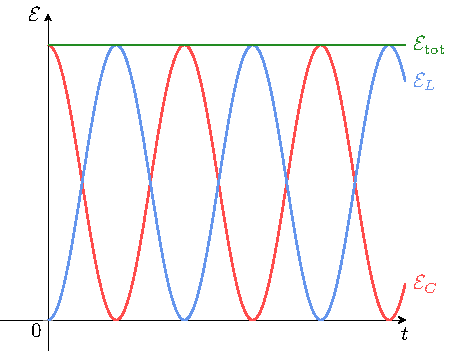
\includegraphics[width=\linewidth,
					draft=true]{carac-lc_descendant-bilan}
			}{
				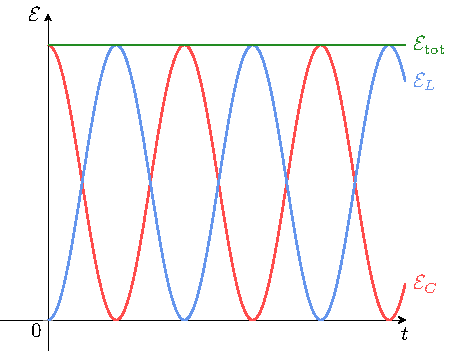
\includegraphics[width=\linewidth]{carac-lc_descendant-bilan}
			}
			\captionof{figure}{}
		\end{center}
	\end{isd}
  \nitem{2} Tracer les solutions $u_C(t)$ et $i(t)$ dans l'\textbf{espace des
  phases} (axe $x = u_C(t)$, axe $y = i(t)$), et \textbf{indiquer le sens de
  parcours}. Expliquer succinctement pourquoi on obtient cette forme.
  \smallbreak
  \begin{isd}[lefthand ratio=.25]
		\begin{center}
			\switch{
				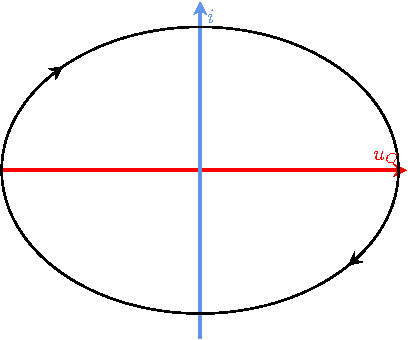
\includegraphics[width=\linewidth,
					draft=true]{carac-rlc_xy-harmo}
			}{
				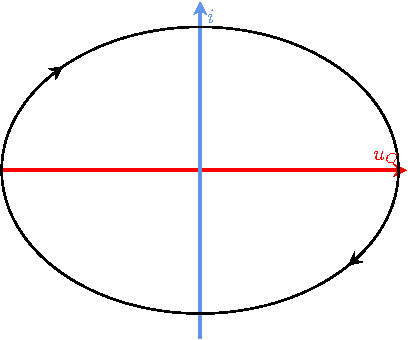
\includegraphics[width=\linewidth]{carac-rlc_xy-harmo}
			}
			\captionof{figure}{}
    \vspace{-15pt}
		\end{center}
    \tcblower
    \wsw{
      On obtient une ellipse étant donné que $u_C(t) \propto \cos(\w_0t)$ et
      que $i(t) \propto \sin(\w_0t)$
      \smallbreak
      Par construction, cela correspond à tracer un cercle déformé puisque
      $\cos^{2}(x) + \sin^{2}(x) = 1$.
    }
  \end{isd}
  \vspace{-15pt}
\end{enumerate}
\end{document}
